\documentclass[12pt]{article}

\usepackage{float}
\usepackage{amsmath}
\usepackage{amsfonts}
\usepackage{subcaption}
\usepackage{graphicx}
\graphicspath{ {./images/} }

\usepackage{listingsutf8}
\usepackage[utf8]{inputenc}

\usepackage[a4paper, total={16cm, 23.7cm}]{geometry}
\DeclareMathSizes{12}{13}{10}{8}
\setlength\parindent{0.7cm}

\usepackage[colorlinks=true,urlcolor=blue]{hyperref}
\usepackage{color}

\newcommand*\diff{\mathop{}\!\mathrm{d}}
\newcommand*\Diff[1]{\mathop{}\!\mathrm{d^#1}}
\newcommand\tab[1][.7cm]{\hspace*{#1}}
\renewcommand{\refname}{}

\captionsetup{width=0.8\textwidth}

\fontfamily{phv}

% !TeX spellcheck = en_US


\begin{document}	
	
	%----------------------------------------------------------------------------
	% TITLE
	%----------------------------------------------------------------------------
	\begin{center}
		\Huge Performance optimization of the online data processing software of CERN's LHCb experiment\\
		\Large Thesis report\\
		\vspace{1pc}
		\huge Péter Kardos \\
		\large 2018-2019
	\end{center}
	
	
	%----------------------------------------------------------------------------
	% === ABSTRACT ===
	%----------------------------------------------------------------------------
	\section{Abstract}
	
	\color{red}
	write at the end \\
	100-200 words \\
	- what's the problem \\
	- how was it solved \\
	- what are the results \\
	- conclusion: what it means for the future \\
	must be understandable without extra info	
	\color{black}
	\vspace{1.5pc}
		
	\textcolor{cyan}{Don't read this, it's just a placeholder.}
	So this abstract should be about 100-200 words so I'm just writing some natural text to act as a placeholder. By looping this text a few times, I can probably make a 150 word section. So this abstract should be about 100-200 words so I'm just writing some natural text to act as a placeholder. By looping this text a few times, I can probably make a 150 word section. So this abstract should be about 100-200 words so I'm just writing some natural text to act as a placeholder. By looping this text a few times, I can probably make a 150 word section. So this abstract should be about 100-200 words so I'm just writing some natural text to act as a placeholder. By looping this text a few times, I can probably make a 150 word section. So this abstract should be about 100-200 words so I'm just writing some natural text to act as a placeholder. By looping this text a few times, I can probably make a 150 word section.
	
	
	%----------------------------------------------------------------------------
	% === Introduction ===
	%----------------------------------------------------------------------------
	\newpage
	\section{Introduction}
	
	\color{red}
	describe the problem in detail \\
	specific to my thesis: \\
	environment: \\
	- CERN's goals/activity \\
	- CERN's hardware infrastructure (accelerators, experiments) \\
	- LHCb's hardware infrastructure \\
	- LHCb's software reconstruction system \\
	problem: \\
	- event rate from detector \\
	- slow trigger $\rightarrow$ loss of physics (ACTUAL PROBLEM) \\
	- by optimizing individual algorithms (in this thesis) \\
	\color{black}
	\vspace{1.5pc}
	
	\subsection{About CERN}
	
	CERN (European Organization for Nuclear Research) is an international high energy experimental physics research organization situated near Geneva, on the Franco-Swiss border. CERN is host to the world's largest particle accelerator and numerous experiments which aim to provide a better understanding of the universe. The goals of the experiments, among others, are to verify the standard model of particles. \textcolor{cyan}{TODO: list more concrete goals}.
	\cite{cern_about}
	
	
	\subsection{The accelerator complex \cite{cern_accel_complex}}
	
	\begin{figure}[H]
		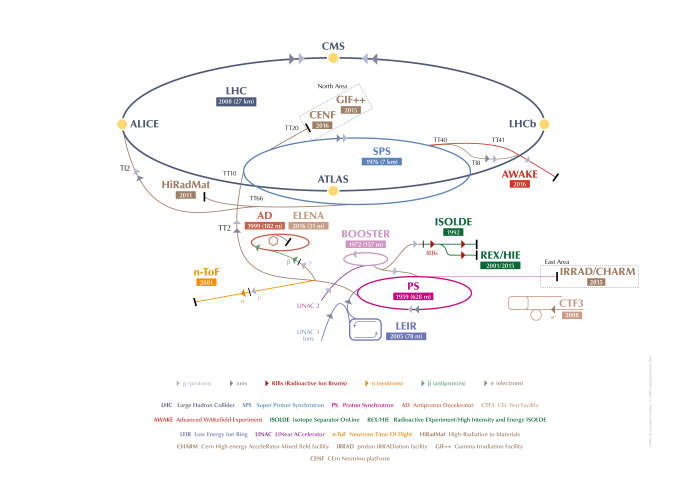
\includegraphics[width=\textwidth]{accelerator_complex}
		\caption{Schematic view of CERN's particle accelerators and experiments. LHC is shown on top by the largest circle. The four main experiments, CMS, ALICE, ATLAS and LHCb are marked with yellow dots along the LHC's circle.}
		\label{fig_accel_complex}
	\end{figure}

	While CERN is mostly known for its Large Hadron Collider (LHC) which this thesis is concerned with, it is home to many more particle accelerators. These accelerators are useful on their own, but from the perspective of the LHC they are used to provide high energy protons that the LHC can further accelerate. Too low energy protons cannot be directly accepted into the LHC, so a sequence of progressively larger accelerators bump the energies up in steps. When a particular accelerator reached its top energy, its beam is simply transferred to a bigger one, finally getting injected into LHC.
	
	The LHC is CERN's largest machine. It can be found inside a circular underground tunnel of a circumference of 27km. There are two accelerators inside the tunnel which accelerate protons so that there is one beam clockwise and another counter-clockwise. Protons are not equally distributed in the beams as they circle around, rather, they can be found in many equally spaced \textit{bunches}.
	
	At specific points along the circle of the LHC, the two beams of opposing directions are made to cross each other's path. As two bunches go through the crossing point at the same time and the individual protons collide\cite{lhc_bunch_collisions}. Since each proton carries around 7 TeV of energy, the collision's yield is about 14 TeV. In the collision, other particles might be born, and that's exactly what scientists are looking forward to analyze.	

	
	\subsection{Experiments on LHC}
	
	As seen on figure \ref{fig_accel_complex}, the four main experiments dedicated to analyze LHC collisions are ATLAS, CMS, ALICE and LHCb. Consequently, these experiments have huge underground rooms around the collisions points, where they can fit their instruments.
	
	The instruments are meant to track and identify particles created in the collisions, and are thus called particle \textit{detectors}. The type and properties of particles created in the collisions provide valuable data to physicists who are trying to verify and extend the standard model of particles. In most cases, the raw data provided by the detectors is processed by software, which does the tracking and identification.
	
	
	\subsection{LHCb's detector}
		
	\begin{figure}[H]
		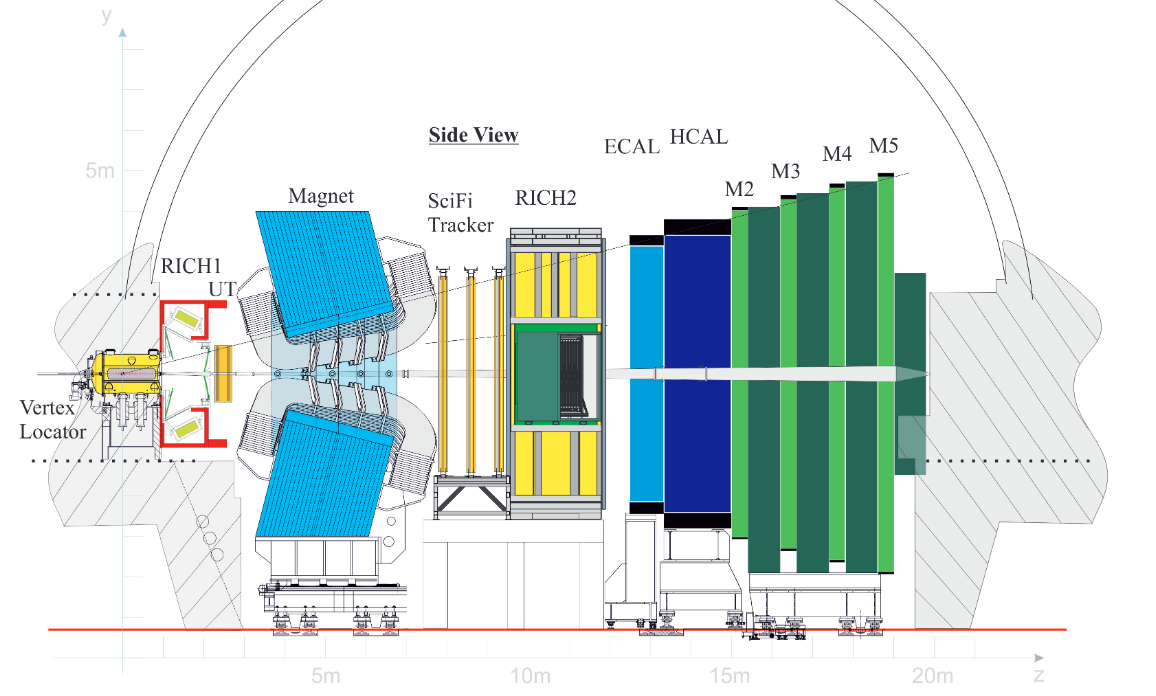
\includegraphics[width=\textwidth]{lhcb_geometry_upgrade}
		\caption{Side view of the LHCb detector.}
		\label{fig_lhcb_geometry}
	\end{figure}

	Figure \ref{fig_lhcb_geometry} shows the LHCb detector from the side, which means that the two beams of LHC are going in horizontal directions on the drawing through the middle of the detector. The middle of the detector coincides with the horizontal axis of symmetry.
	
	As seen on the labels, the detector consists of multiple layers of sub-detectors. Each layer has a hole in the center to let the beam pipes through. The two particle beams cross each other inside the Vertex Locator (VELO, at the right in yellow).
	
	While full reconstruction uses all sub-detectors, real-time reconstruction only uses the VELO, the UT (in orange, left of VELO) and the FT (SciFi Tracker, in the middle in orange). Let's follow the life of a particle from its birth inside the VELO. While flying away from the collision point, it first crosses multiple layers of the VELO. Each layer consists of many pixels, and whenever the particle touches a pixel, the VELO forwards this information to the software. Eventually, the particle leaves the VELO and goes through the UT. The UT has a different mechanism compared to the VELO, but essentially it also records if a particle has gone through one of its layers. Leaving the UT, the particle goes through the large magnet, where its path is bent due to the Lorentz force by an amount dependent on its electric charge and momentum. The particle then keeps going straight through the FT, where its location is registered as usual. Note that for each bunch collision, hundreds of new particles go through the detector as described above. The reconstruction software tries to make sense out of the large number of registered particle positions by using knowledge about the magnetic field, and eventually identifies the individual particles and their tracks.
	
	The purpose of real-time (sometimes called \textit{online}) reconstruction is to determine what data to store. Most collision events are not interesting at all from a physics perspective, and only a small fraction is kept for long-term storage. Storing all data would be unfeasible because of its sheer amount. The software doing the online reconstruction and selection is called the \textit{trigger}.
	
	\subsection{The 2018/19 upgrade of LHCb}
	
	The catch with the above described detector is that it does not really exist yet. The LHC will be shut down in 2018 december for maintenance, and that's when the LHCb collaboration will upgrade its detector to the one above. (The current detector is similar in construction, that's why it's referred to as \textit{upgrade}.)
	
	With the upgrade, software data processing will change significantly as well. Around 30 million bunch collision events occur every second, each of which go through the trigger. With the current detector, triggering is first done by hardware electronics, selecting only 1 million events per second, which are then further culled on a big server farm by software written in C++. After the upgrade, the hardware trigger is dropped and the entire trigger runs in software. This puts the high requirement on the software trigger to reconstruct and cull all the 30 million events every second.
	
	\begin{figure}[H]
		\centering
		\begin{subfigure}{.5\textwidth}
			\centering
			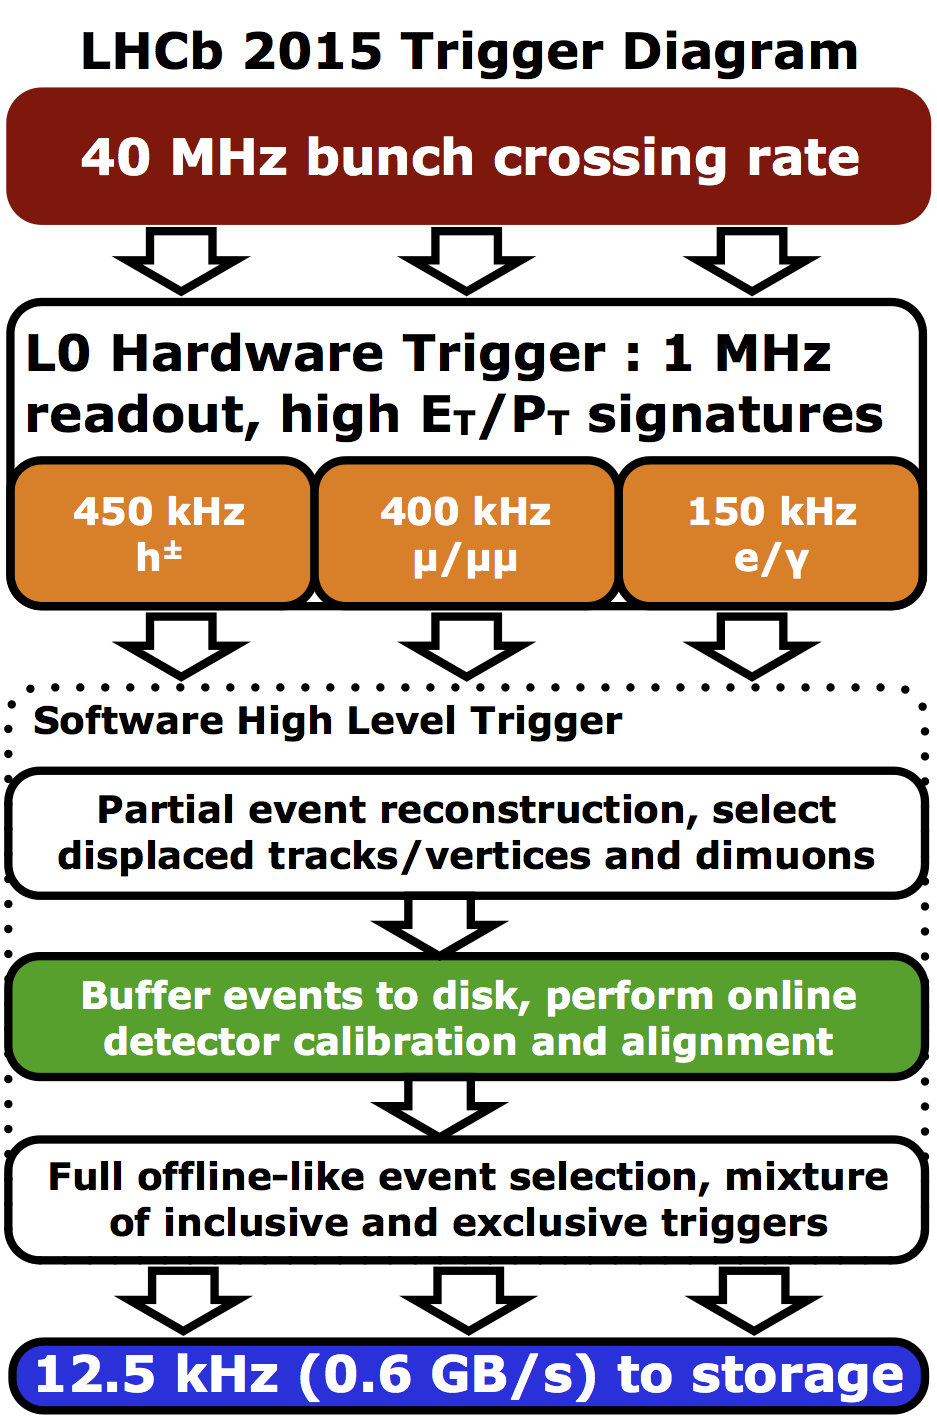
\includegraphics[width=.4\linewidth]{LHCb_Trigger_RunII_May2015}
			\caption{Trigger data flow scheme\\ before the upgrade}
			\label{fig:sub1}
		\end{subfigure}%
		\begin{subfigure}{.5\textwidth}
			\centering
			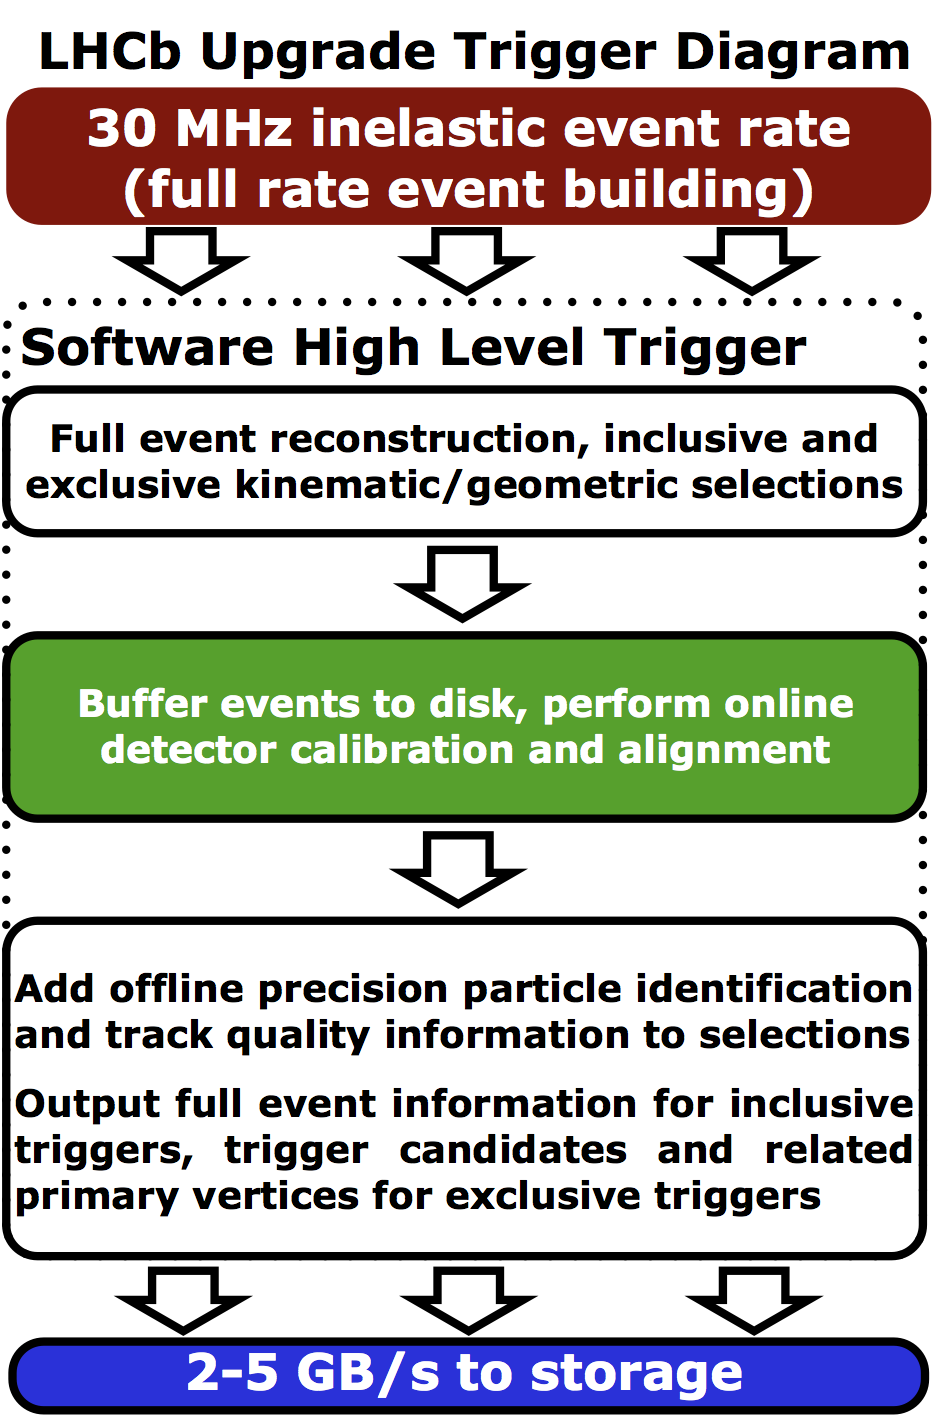
\includegraphics[width=.4\linewidth]{LHCb_Trigger_RunIII_May2015}
			\caption{Trigger data flow\\ scheme post-upgrade}
			\label{fig:sub2}
		\end{subfigure}
		\caption{Comparison of the two triggering solutions}
		\label{fig_trigger_compare}
	\end{figure}
	
	
	\subsection{Overview of the trigger software}
	\label{intro_algos_overview}
		
	\begin{figure}[H]
		\begin{center}
			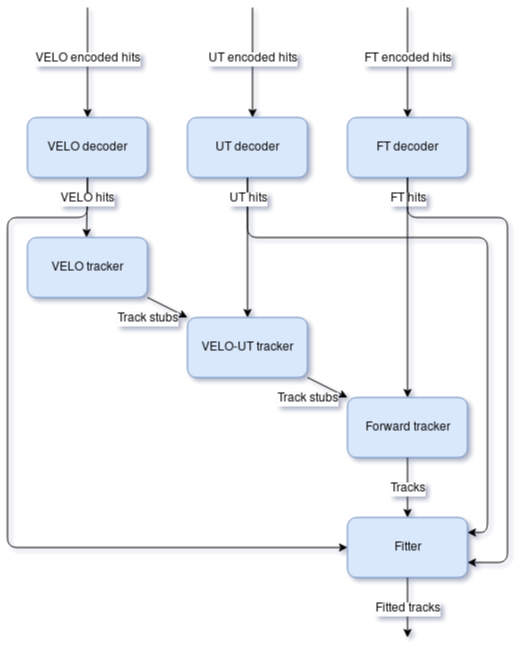
\includegraphics[width=0.6\textwidth]{algorithms_brunel}
		\end{center}
		\caption{Simplified view of algorithms that perform online reconstruction.}
		\label{fig_algorithms_brunel}
	\end{figure}


	The trigger software is basically the online reconstruction code and additional logic to select which events to keep. The online reconstruction software can be broken down to individual pieces referred to as \textit{algorithms}, each of which serves a specific purpose. First of all, the highly compressed data that arrives from the detector has to be decoded to acquire hits that describe the position and measurement error of points where a particle has been seen. Second, the particles' tracks are progressively reconstructed by starting from the collision point in the VELO, and appending hits to an existing track. In the VELO and UT, we are looking for hits that form a straight line, and we try to match this straight track to another similarly straight track inside the FT. Finally, the track goes through fitting, which tries to modify the existing rough track to more closely line up with the hits it was produced from.
	

	\subsection{The aim of this thesis project}
	
	As mentioned, the abandoning of the hardware trigger stage highly increases the load on the software trigger. The main goal of this project is to optimize the current software trigger to make it about 3 times as fast. Failure to do so will result in valuable events being dropped, thus reducing the physics potential of the experiment.
	
	Current computing hardware has changed significantly from the ones the software trigger was originally made for. The even larger gap between memory and CPU speeds demands a more efficient use of CPU caches. Additionally, CPU instruction sets now include SIMD operations, which can, for example, do 4 floating point operations in place of one in the same amount of time. Furthermore, modern CPUs have a complex logic for branch prediction and instruction pipelining, which require code to be tailored to serve them.

	To exploit the full capability of current hardware, not only individual pieces of the trigger software need to be changed, but the global data flow also has to be rethought and optimized.
	
	During this thesis project, I will be helping the LHCb collaboration to reach its optimization goals for the software trigger.
	
	%----------------------------------------------------------------------------
	% === TBD ===
	%----------------------------------------------------------------------------
	\newpage
	\section{Choosing optimization targets}
	
	\color{red}
	Explain the choice of initial choice of algorithms, based on the pie chart diagram and logical reasoning of our goals (i.e. what's needed).
	\color{black}
	
	As mentioned in \ref{intro_algos_overview}, the reconstruction consists of individual algorithms which account for the bulk of the computation. (Scheduling the algorithms and culling decisions account for a much smaller CPU load.) It is straightforward to first start optimizing the algorithms which take the largest chunk of available computing power.
	
	\begin{figure}[H]
		\begin{center}
			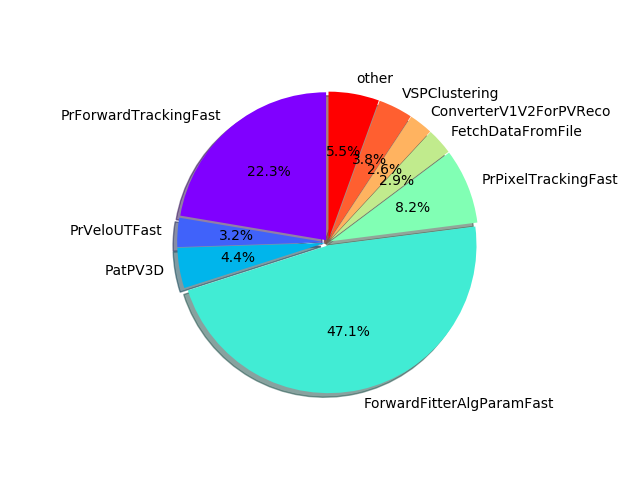
\includegraphics[width=0.6\textwidth]{algo_usage_original_bestphys}
		\end{center}
		\caption{Workload split among HLT1 algorithms.}
		\label{fig_algo_usage_choice}
	\end{figure}

	Looking at figure \ref{fig_algo_usage_choice}, we can see that the parametrized Kalman fitter takes nearly half the CPU budget, followed by the forward tracking which takes roughly a quarter. Based on this and initial performance profiling of the algorithms for hotspots, I decided to first examine and optimize the Kalman fitter. 
	
	%----------------------------------------------------------------------------
	% === TBD ===
	%----------------------------------------------------------------------------
	\section{Parametrized Kalman Fitter}
	
	As described in \ref{intro_algos_overview}, the track is reconstructed incrementally, start with velo hits, extended by UT hits and finally adding the FT hits. This process, however, is not so accurate. This manifests itself in the creation of \textit{ghost tracks} and missed tracks, and generally, tracks are only roughly aligned with the hits they were made from. Ghost tracks are tracks that did not exist in the real collision, they are merely artifacts of the reconstruction algorithms. As such, ghost tracks are highly undesirable, but this is where the Kalman fitter comes into play. 
	The Kalman fitter basically refines the rough tracks that are spit out by preceding algorithms. The state of a particle can be described by its position, direction, and the quotient of its charge and momentum. The Kalman fitter first estimates the particle's state at its birth position based on the Velo hits alone. After that, it extrapolates the state of the particle to the next hit, or in other words, simulates the particle's travel until the next hit using the laws of physics. The new, \textit{predicted} state will have some deviation to the \textit{observed} state (that is, the hit), however, the Kalman fitter can make a mathematically optimal estimate for the true state based on the prediction and observation. The very new optimal state estimate will then be extrapolated to the next hit again, and this repeats for all the hits of the track.
	As a result, the estimated state or path of the particle aligns more closely with the observed hits. In the case of ghost tracks, we can expect to have large deviations between the optimal estimated states and the observed hits, which could slipped through initial reconstruction algorithms but show up for the fitter. Such tracks are removed from the list of tracks, and that's why fitting is important.	
	
	\subsection{Performance profiling for hotspots}
	
	\textcolor{red}{TODO: Add the actual vtune screenshot.}
	\begin{figure}[H]
		\begin{center}
			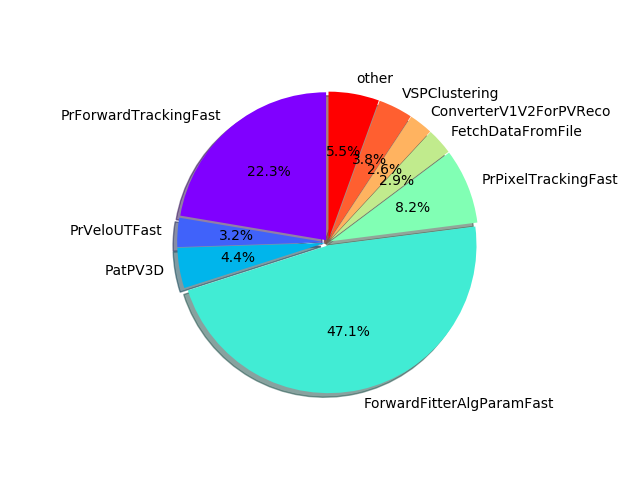
\includegraphics[width=0.6\textwidth]{algo_usage_original_bestphys}
		\end{center}
		\caption{Code hotspots as measured by Intel VTune Amplifier XE.}
		\label{fig_kalman_vtune_initial}
	\end{figure}
	
	Figure \ref{fig_kalman_vtune_initial} shows what fraction of the CPU time is spent in each individual function of the code. We can nicely see how the theoretical steps of the Kalman fitting map to the functions:
	\begin{itemize}
		\item LoadHits: acquires position and measurement error of hits
		\item PredictState: extrapolates the state to the next hit
		\item UpdateState: makes an optimal estimate for the true state using the predicted state and the measured hit
		\item AverageState, ExtrapolateToVertex, etc.: various operations
	\end{itemize}
	There is a major and obvious problem however: just acquiring the data on which the computation is done should not take over 50\% of the Kalman fitting, but more like 1\%.	
	
	\subsection{Examination of the }
	
	\subsection{Evaluation of results}
		
	
	%----------------------------------------------------------------------------
	% === TBD ===
	%----------------------------------------------------------------------------
	\section{TBD}
	
	%----------------------------------------------------------------------------
	% === Conclusion ===
	%----------------------------------------------------------------------------
	\section{Conclusion}
	
	\color{red}
	- summarize my own contributions \\
	- summarize achieved results \\
	- make conclusions about them \\
	- how it affects the future \\
	BRIEFLY
	\color{black}

	
	%----------------------------------------------------------------------------
	% REFERENCES
	%----------------------------------------------------------------------------
	\section{References}
	
	\begin{thebibliography}{asd}
		\bibitem{cern_about} About CERN: \\
			\url{https://home.cern/about}
		\bibitem{cern_accel_complex} The accelerator complex: \\
			\url{https://home.cern/about/accelerators}
		\bibitem{lhc_desc} About the Large Hadron Collider: \\
			\url{https://home.cern/topics/large-hadron-collider}
		\bibitem{lchb_desc} About the Large Hadron Collider beauty experiment: \\
			\url{https://home.cern/about/experiments/lhcb}
		\bibitem{lhc_lead_ions} Why collide lead ions: \\
			\url{http://alicematters.web.cern.ch/?q=FAQ-why-lead-ions}
		\bibitem{lhc_energy} Energy of the LHC: \\
			\url{https://home.cern/about/engineering/restarting-lhc-why-13-tev}
		\bibitem{lhc_bunch_collisions} https://lhc-machine-outreach.web.cern.ch/lhc-machine-outreach/collisions.htm
	\end{thebibliography}

\end{document}





















